


\section{Pirate Game}
\label{sec:pirate}

\begin{emph}
On selecting the problem...
\end{emph}


\subsection{Problem Description}
\label{subsec:description}

The original Pirate Game is a multiplayer version of the Ultimatum game that is usually stated as follows:

\begin{quotation}
Suppose there are 5 rational pirates: A; B; C; D; E. The pirates have a  loot of 100 indivisible gold coins to divide among themselves.


As the pirates have a strict hierarchy, in which pirate A is the captain and E has the lowest rank, the highest ranking pirate alive will propose a division. Then each pirate will cast a vote on whether or not to accept the proposal. 

If a majority or a tie is reached the goods will be allocated according to the proposal. Otherwise the proposer will be thrown overboard and the next pirate in the hierarchy assumes the place of the captain. 

We consider that each pirate privileges her survival, and then will want to maximize the number of coins received. When the result is indifferent the pirates prefer to throw another pirate overboard and thus climbing in the hierarchy. 
\end{quotation}

We can arrive at an equilibrium in this problem by using backward induction. At the end of the problem, supposing there are two pirates left, the decisions are very straight forward. As the highest ranking pirate can pass the proposal without the remaining friend, her self-interest dictates that she will get the 100 gold coins. Knowing this, pirate E knows that any bribe other higher ranking pirate offers her will leave her better than if the game arrives to the last proposal. 

\begin{table}
\begin{center}
\begin{tabular}{cc}
  \num\putindeepbox[7pt]{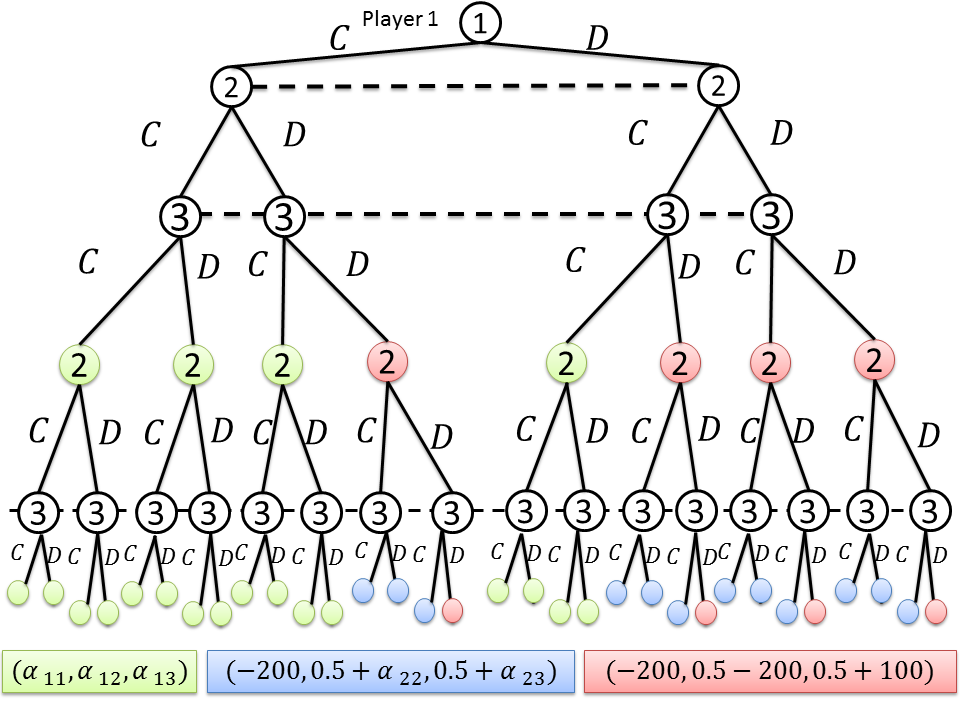
\includegraphics[scale=0.20]{Pirates1/Slide1.PNG}}
    & \num\putindeepbox[7pt]{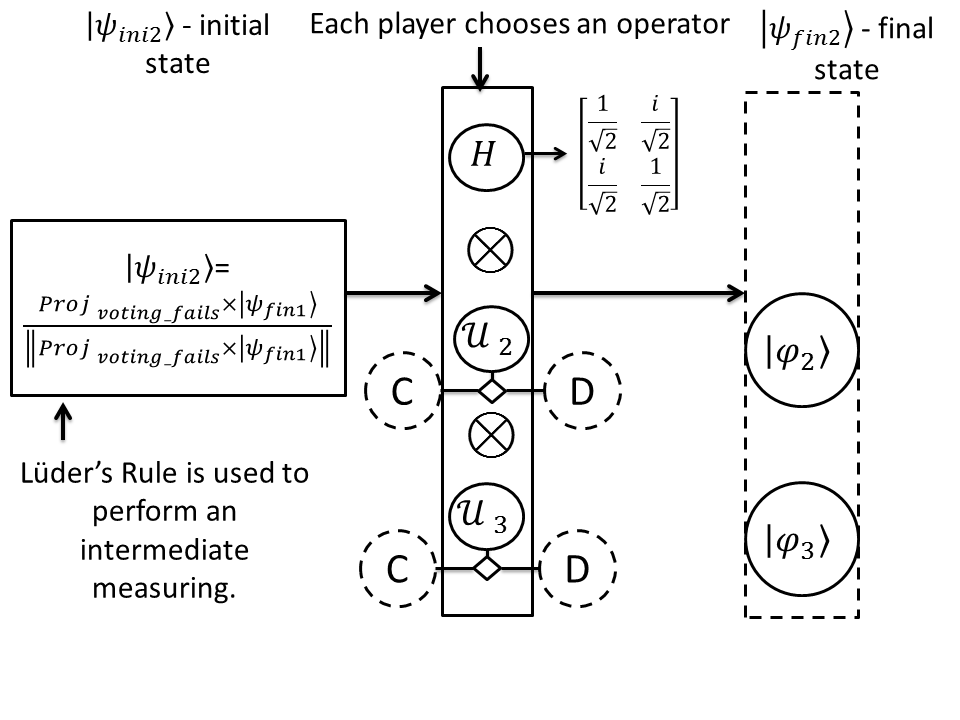
\includegraphics[scale=0.20]{Pirates1/Slide2.PNG}} \\
  \num\putindeepbox[7pt]{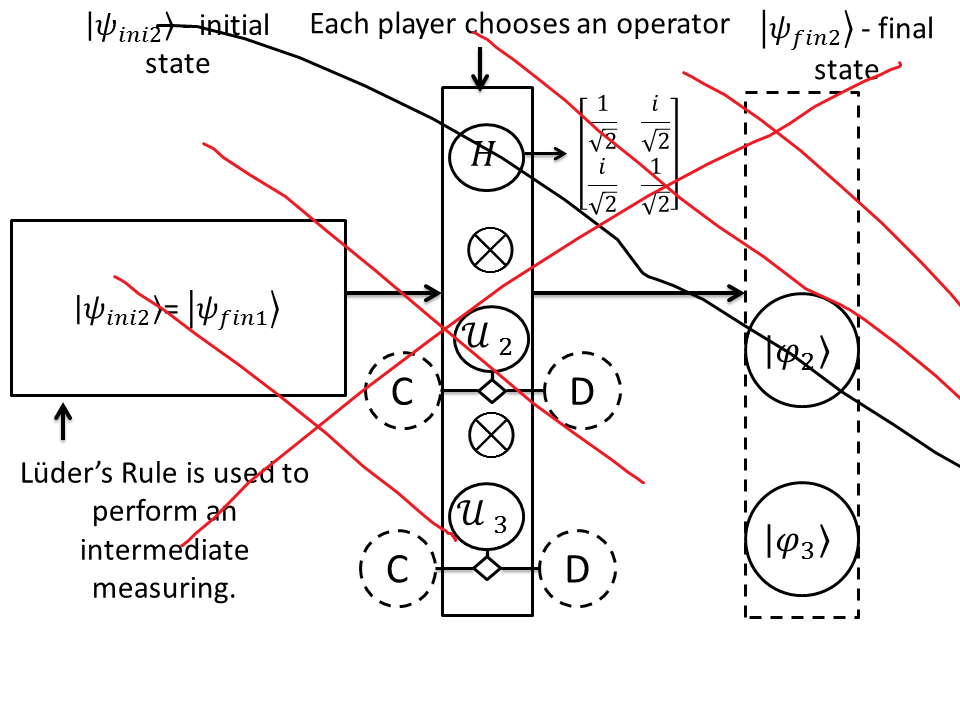
\includegraphics[scale=0.20]{Pirates1/Slide3.PNG}}
    & \num\putindeepbox[7pt]{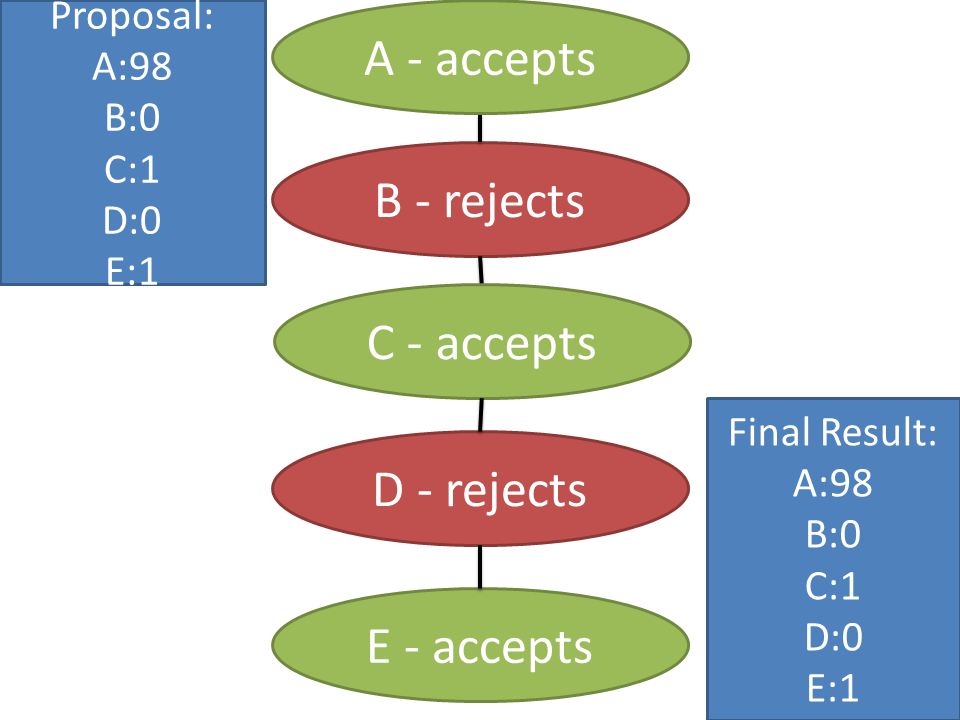
\includegraphics[scale=0.20]{Pirates1/Slide4.PNG}} \\
\end{tabular}
\caption{The equilibrium for the Pitrate Game can be found through backward induction. From a), where there's only two pirates left, to d), that corresponds to the initial problem we define the best response.}
\label{tab:piratas_m}
\end{center}
 \end{table}

When applying this reasoning to the three pirate move, as pirate C knows she needs one more vote to pass her proposal and avoiding death, she will offer the minimum amount of coins that will make pirate E better off than if it comes to the last stage with two pirates. This means that pirate C will offer 1 gold coin to pirate E, and keep the remaining 99 coins. 

With 4 pirates, B would rather bribe pirate D with 1 gold coin, because E would rather like climb on the hierarchy and getting the same payoff. Finaly, with 5 pirates the captain (A), will keep 98 gold coins and rely on pirate C and E to vote in favor of the proposal, by giving 1 gold coin each.

We can generalize this problem for $N$ pirate. If we assign a number to each pirate, where the captain is number 1 and the lower the number the higher the rank. If the number of coins is superior to the number of pirates, the equilibrium will have the captain (highest ranking pirate), giving a gold coin to each odd pirate, in case the number of players alive is odd, while keeping the rest to herself. When we have a even number of players the captain will assign a gold peice to each pirate with a even number, and the the remaining coins to herself.




\subsection{Quantum considerations}
\label{subsec:description_2}

In order to model the mencioned problem it's helpful to define it using the definition \ref{eq:quantum_game_six_tuple} in Section \refl{sec:background_quantum_game_theory}.
In terms of mechanics and steps, this problem could be described using 3 players and later extended to any number $N$ of players. We will assign an offset to each pirate in order to identify it, as in the Section \label{subsec:description}. So the captain is number 1 and the lower the number the higher the rank. 

Each player will be able to manipulate a qubit.




 The highest ranking pirate in the hierachy will be responsible to make a proposal. This proposal can be modelled as describing the payoff functionals for every pirate, according to some rules. This goods allocation proposal will be executed if there is a majority (or a tie), in the voting step. In the voting step, each pirate will cast a vote by choosing simultaneously a operator (that can mean either accep or reject the proposal).
''''''Depending on the measurement outcome that occurs with probability x, the players will act on the second round. The Luders rule is applied here. The highest ranking player will no longer have access to the YES or NO operatos, instead he will only be able to manipulate de system using a symetric matrix like a coin operator, in order to not affect the voting.

Keeping the system in a higher dimension is considered because of the following reasons: We don't have proof that the states are separable. There are various mappings that fit the system composition. 


Initial state: variable to study.
Payoff functions: variable to study.

\begin{emph}
One important aspect is that the payoff functional changes
\end{emph}